% Use the temporary template.
\documentclass[]{aiaa-pretty}

%Packages
\usepackage{subfigure}
\usepackage{amsmath}
\usepackage{graphicx}
\graphicspath{{./pics/}}
\usepackage{mcode}

% Author information
\author[Vascik, Wald, and Ward]{ %
Parker Vascik\thanks{Doctoral Student, Department of Aeronautics \& Astronautics, \texttt{pvascik@mit.edu}},
Samuel Wald\thanks{Doctoral Student, Department of Aeronautics \& Astronautics, \texttt{swald@mit.edu}},
Eric Ward\thanks{Systems Design and Management Fellow, Institute for Data, Systems and Society, \texttt{ericward@mit.edu}}\\
\textit{Massachusetts Institute of Technology, Cambridge, MA 02139}}

% Title
\title{Mars Outpost Resupply Optimization}


% Abstract
 \abstract{ %
This paper presents an analysis of the effects of various campaign and mission architecture decisions for a permanent Martian surface outpost on the resulting resupply requirements in an effort to improve the overall campaign's sustainability. The investigation includes quantification of outpost technology development costs, resupply launch costs from Earth, and scientific value provided from the Martian surface. Multi-objective, multi-disciplinary system optimization is used as a primary method of trade-space exploration and characterization. A final design recommendation is provided that balances competing objectives. It is shown to be a Pareto-dominant architecture defined by crew size, in-situ food production, and propulsion capabilities. This work stands as an example of how integrated system analysis can be used to aid decision makers in mission planning on technology development road-mapping with future uncertainties.}

% Conference name
% NOTE: This will not appear unless the 'journal' option is selected.
% NOTE: This will not appear if a journal is specified
\conference{nth Conference on MDO\\
24 July 1687, Cambridge, Massachussetts}
% NOTE: This will not appear unless the 'journal' option is selected.
% Paper number that couldn't exist
\papernumber{AIAA 1687-45A2}

% Journal name
\journal{Journal of Anachronistic Computers}

% Volume
\volume{Vol.~0, No.~0, June--July}

% DOI
%\doi{10.2514/6.1687-45A2}

% Copyright
\copyright{Copyright \textcopyright 2016 Massachusetts Institute of Technology}

% Begin the document
\begin{document}
% Insert the title.
\maketitle

\section{Nomenclature}
\begin{table}[]
\centering
\label{tab:Nom}
\begin{tabular}{lll}
x   & = & design vector                \\
\( \alpha \)   & = & 5.65 x 10-4                  \\
\( \beta \)   & = & 0.5941                       \\
\( \Xi \)   & = & 0.6604                       \\
\( \delta \)   & = & 80.599                       \\
\( \varepsilon \)   & = & 3.8085 x 10-55               \\
\( \phi \)   & = & -0.3553                      \\
\( \gamma \)   & = & 1.5691                       \\
Q   & = & Quantity                     \\
M   & = & Dry Mass (lbs)               \\
S   & = & Specification                \\
IOC & = & Initial Operating Capability \\
B   & = & Block Number                 \\
D   & = & Difficulty                  
\end{tabular}
\end{table}


\section{Motivation}
\label{sec:Motivation}
The United States and its international partners are on a “Journey to Mars” with the explicit goal of changing moving from Earth-reliant to Earth-independent space system architectures within the century. \cite{craig2015pioneering} There are many potential sources of value from such an endeavor; the two most emphasized in the analysis presented here are to 1) enhance our current scientific understanding of the biological and geological history of the solar system and 2) provide a safe haven to ensure long-term human survival. \cite{NRC2014} These objectives will require large investments of resources to development the necessary technologies and launch them to the Martian surface to sustain a stable population indefinitely. 

In 2015 a team of graduate system design and management students at the Massachusetts Institute of Technology developed a framework and element models to generate and evaluate system architectures that could enable a sustained presence on Mars with varying levels of resupply required from Earth by the year 2040. Their analysis focused on simulating the steady-state logistics and supporting infrastructure necessary to transfer supplies from Earth or produce them in-situ. Architectures were evaluated based on total mass in low-Earth orbit (a proxy for cost) and the scientific value that could potentially be derived from the population on the Martian surface. Their efforts produced a model of a Mars outpost architecture including the transportation logistics, surface habitation, ISRU and exploration aspects. A tradespace exploration was conducted spanning a variety of potential input values to identify architectures that minimized the IMLEO (initial mass to low-earth orbit, i.e. the total payload launched from the Earth surface each synodic period) while attempting to maximize the scientific value as defined as the crew-hours per synodic period available for exploration and research, multiplied by a rank scoring of the landing sites.

The analysis presented in this paper builds upon these previous efforts' work by adding design objectives and modeling capability representing technology investments, their development costs, launch costs to LEO, and total scientific return on investment. Advanced transit propulsion systems, including nuclear thermal rockets and extremely high specific impulse chemical rockets, and ISRU technologies were investigated as potential high impact developments supporting potential missions to Mars. The expanded design space is well-suited for multi-disciplinary, multi-objective, system optimization. The model and optimization advancements made through this research are the next step in ensuring that the chosen Mars 2040 architecture is not only feasible, but Pareto-optimal within the constraints of physical and financial limitations. 

\section{Problem Formulation}  
\label{sec:formulation}
The primary goal of this analysis is to optimize the steady-state performance of a permanently inhabited outpost on the surface of Mars subject to technology development and operational cost  considerations. Various design variables associated with technological performance are varied to capture and compare different investment options, as well as simulate uncertainty in paramaters such as launch costs. The following sections describe the formal problem definition for optimization including objectives, design variables, constraints, parameters and assumptions.

\subsection{Objectives}
The chosen formulation is that of a minimization problem with up to three objectives. These are: 
\begin{enumerate}
\item Scientific Utility (negative): the number of crew-person-hours available to perform scientifically valuable tasks on the Martian surface. The utility of each hour is weighted by the scientific interest at each location, where some landing sites have greater potential scientific value (perhaps at the cost of more stringent ISRU requirements). Note that the optimization problem will seek to \textit{maximize} the scientific utility of the mission. Therefore, the objective shall be to minimize the negative of scientific utility. This method is based on the utility metrics presented in recent work of Ward et. al. \cite{ward2015}.
\item Resupply Cost: the cost, in millions of 2016 equivalent dollars, to launch the required resupply mass from the Earth to LEO.
\item Development Cost: the cost, in millions of 2016 equivalent dollars, to develop new or improve existing select technologies.
\end{enumerate}
The details of how each of these objectives are calculated in order to evaluate and search amongst architectures are presented in Section \ref{sec:model}. 

\subsection{Design Variables}
\label{sec:DVs}
The Mars 2040 design space was expanded to include new design variables that are expected have a significant efect on the value of the three objective functions. These design variables were selected through senstivity studies on the original SDM team design space to identify paramaters that had a large influence on the science utility of the final selected architecture. These paramaters were then converted to design variables in this analysis in an attempt to find a more optimal soltuion. The new design variables considered in this analysis are:
\begin{enumerate}
\item LH$_2$ Isp: the specific impulse of the chemical transit propulsion (liquid oxygen/hydrogen rockets) stage used for each resupply mission.
\item NTR Isp: the specific impulse of the NTR transit propulsion stage used for each resupply mission.
\item Surface Population: the minimum number of people on the Martian surface at any time. The population increases during each hand-off.
\end{enumerate} 
Lunar ISRU efficiency was also initially considered as a design variable for this analysis due to the criticality of the technology in the various Mars campaign architectures. Recent studies have shown the potential benefits of obtaining transit propellant from the lunar surface, and that this benefit is highly sensitive to the mass efficiency of the mining and processing systems necessary to produce it \cite{ho2014dynamic}]. However, as the analysis presented in this paper is limited to resupply cost and does not include the initial emplacement cost as part of the objective, technology investments in varying levels of ISRU efficiency did not have a significant impact upon the chosen campaign objectives. For this reason, technology investments in ISRU efficiency were not included in the problem formulation presented here but it is recommended they be considered in future work as discussed in Section \ref{sec:single}). This analysis did consider the type and location of ISRU as a design variable, however, as the use of ISRU dramatically influences the resupply propellant requirements and IMLEO. Therefore, the mission architecture is optimized for either no ISRU, mixed lunar/Martian and Earth ISRU, or full lunar/Martian ISRU.

\subsection{Constraints and Bounds}
\label{sec:constraints}
Constraints are dictated by the physics of the Mars 2040 campaign problem including aspects such as supplying the necessary propellant to transport materials to and from Mars, producing adquate power for each outpost element on the Martian surface, and ensuring a mass balance of consumables such as air, water, and food for the crew. 

Beyond these physics based constraints on the mission architecture, bounds were applied to each of the problem design variables to capture technology development limitations and reasonable crew sizes. For the two propulsion specific impulse independent variables, their feasible ranges are bound between the current state of the art and the theoretical upper limit that could possibly be achieved. The surface population is limited integer numbers between 12 and 30 crew members in order to capture a representative design space for a permanent surface settlement which could be feasible within the timeframe of two to three decades.

\subsection{Problem Statement}
\label{sec:problemstatement}
\begin{equation*}
\mbox{Minimize } J(\mathbf{x})
=
\begin{bmatrix}
\mbox{C}\\
\mbox{-S}\\
\end{bmatrix}
=
\begin{bmatrix}
\mbox{Total Cost (\$M)}\\
\mbox{-Science Utility (scaled person-hours)}\\
\end{bmatrix}
\end{equation*}

\begin{equation*}
\mbox{where } \mathbf{x}
=
\begin{bmatrix}
\mbox{Propulsion Type}\\
\mbox{Propulsion Isp}\\
\mbox{Surface Power Source}\\
\mbox{Outpost Location}\\
\mbox{Food Percentage Grown On Mars}\\
\mbox{Outpost Population}\\
\mbox{Transit Fuel Source}\\
\mbox{Return Fuel Source}\\
\mbox{Entry Type}\\
\mbox{Staging Location}\\
\end{bmatrix}
=
\end{equation*}
\begin{equation*}
\begin{bmatrix}
\mbox{ LH$_2$; NTR}\\
\mbox{ LH$_2$: 445 - 480s; NTR: 850 - 1000s}\\
\mbox{Solar; Nuclear; Fuel Cell}\\
\mbox{Holden; Gale; Meridiani; Gusev; Everswalde; Isidis; Elysium; Mawrth; Utopia; Planus Boreum; Hellas; Amazonis}\\
\mbox{0 to 100\%}\\
\mbox{12 to 30 people}\\
\mbox{Earth, Moon}\\
\mbox{Earth, Mars}\\
\mbox{Aerocapture; Propulsive}\\
\mbox{LEO; EML1; EML2}\\
\end{bmatrix}
\end{equation*}

\subsection{Parameters}
\label{sec:params}
The system model requires the assignment or estimation of multiple parameters and constants that define various aspects of the system. These include material properties, propulsion stage mass fractions, processing efficiencies, equivalent mass factors, and launch cost rates, among other. Sensitivities to some of the key parameters are also investigated and discussed in the results section of this report. A full list of the parameters used for this study may be accessed through the corresponding author. 

\section{Modeling and Simulation}
\label{sec:model}


\subsection{Mission Architectural Element Sizing Model}
\begin{figure}[h!]
	\centering
	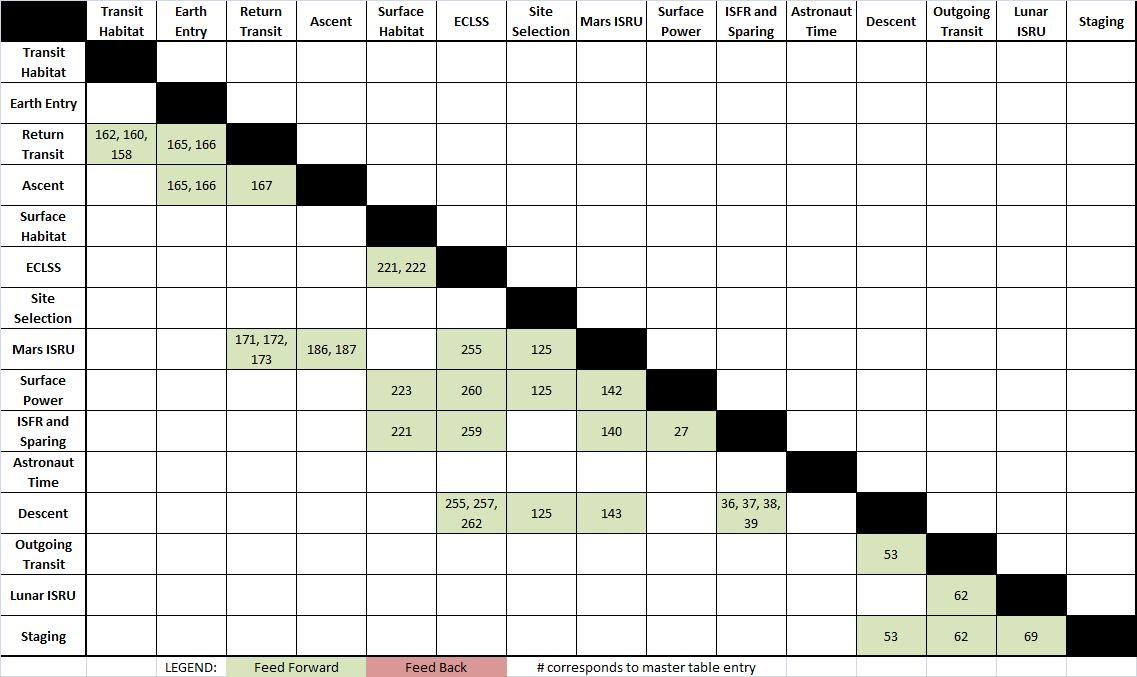
\includegraphics[width=0.7\textwidth]{OrderedDSM}
	\caption{Ordered DSM for outpost and resupply system.}
	\label{fig:orderedDSM}
\end{figure}
This research adds an optimization routine, two additional cost modules, and a more robust scientific value measure the Mars 2040 project that was initiated during Spring 2015 as the SDM term project.  This previous project developed a model to size a Mars outpost resupply mission architecture including the Transportation Logistics, Surface Habitation, ISRU and Exploration aspects. 

This model allows sizing of the mission elements based on the architectural design of the campaign. Figure \ref{fig:orderedDSM} shows a calculation-ordered design structure matrix (DSM) for the initial model. Each module is listed across the top and side, and the inside of the matrix describes the information and variables that are output from one module and input into another. 

\subsection{Scientific Utility Model}

One of the primary motivations for developing a Martian outpost is the scientific knowledge that can be gained by allowing humans to explore the region. Mars is of great interest to multiple scientific communities as evidenced by the significant effort devoted to robotic surface and satellite missions; NASA alone has six currently active missions to learn more about the planet. \cite{nasa2016mars} This analysis quantifies the amount of potential valuable scientific data that could be acquired based on a model presented by Ward et. al. \cite{ward2015} The model incorporates two aspects that drive scientific value of the mission: scientific interest in the neighborhood of the outpost and the amount of available crew time to perform scientific tasks.

Site selection is a key decision for future human expeditions to Mars, especially when investing in a permanent facility which will allow astronauts to explore much of the region in great detail. For each of the twelve outpost locations considered, two scientific weighting factors - biological interest and geological interest - were used to assign relative potential of each site. The details of how the factors were determined is discussed by Ward et. al. \cite{ward2015} However, it is noted here that we expect the optimal solution to be sensitive to these weighting factors, and improvements to the method should also be investigated in future work.

Choosing a highly scientifically interesting site will serve little purpose if the outpost population has little time to devote to exploring, sampling, and analyzing the area. A simple model has been used to quantify this available time by calculating the total person-hours available after tending to other labor-intensive duties (e.g.crop management or habitat maintenance). The assumption is made that there is no limit to the scientific activities that could be done, so the value of any particular site scales linearly with increasing time to explore. 
The Scientific Utility Model is thus summarized as:
\begin{equation*}
S=(B_i + G_i) P t
\end{equation*}
where
\begin{equation*}
B_i = \text{Biological Interest Factor of Site i}
\end{equation*}
\begin{equation*}
G_i = \text{Geological Interest Factor of Site i}
\end{equation*}
\begin{equation*}
P = \text{Outpost Population (no. of people)}
\end{equation*}
\begin{equation*}
t = \text{Science Activity Time (hours per person)}
\end{equation*}

\subsection{Cost Model}
Perhaps the most critical constraint on achieving the Mars 2040 mission is the significant, nation-level investment in technology development and production that is necessary to develop a Mars campaign. For reference, in 2016 dollars, the lunar campaign Apollo programs of the 1960’s are estimated to have cost 108 billion dollars \cite{stine2008crs}, the 30 year space shuttle program is estimated at 217 billion dollars, and the development and operation of the international space station thus far is estimated to have cost 150 billion dollars \cite{lafleur2010costs}. Resultantly, these major space programs represent some of the greatest single non-war investments of the United States and required exceptional political will to implement. The Mars 2040 mission is likely to be at or above the level of investment of these previous programs. It is therefore essential that the minimization of the various costs of the Mars 2040 campaign is explicitly considered as a key objective during the conceptual design and optimization phase.

This research elected to consider two categories of costs the Mars 2040 campaign will encounter. The first type of costs are operational costs. Operational costs include all costs incurred during the actual execution of the mars 2040 campaign. The single greatest operational cost of the campaign is the earth launch vehicle construction and earth to orbital staging area launch costs. These two costs are captured in the optimization problem as the “Initial Mass to Low Earth Orbit”, or IMLEO cost. 

The second type of cost considered in this optimization represents the long-term investments made in technology development leading up to (and perhaps throughout) the launch of the Mars 2040 campaign. A significant proportion of the Apollo program costs were accounted for in the development of fundamentally new launch vehicle, space transportation, life support, navigation and computing technologies, among many others, that were necessary for the achievement of the moon landings. Similarly, a Mars campaign may lead to considerable investments and developments in requisite technologies such as advanced propulsion, In-Situ Resource Utilization (ISRU), long duration space flight, and planetary landing vehicles, among others, for example. The long-term investments required to develop such technologies will likely be a significant percentage of the expenditures of a Mars campaign. Therefore, this research shall estimate an “advanced technologies development cost” specifically for improved propulsion technologies and consider this cost within the optimization problem. 

\subsubsection{IMLEO Cost Estimating}
In order to maximize the science return for the mission, we calculated a launch cost based on a constant rate measured in dollars per mass to IMLEO. We chose use the conservative estimate of \$10k/kg based on historical systems as a baseline. However, recent developments in both public (e.g. SLS) and prirvate sector (e.g. SpaceX) launch systems have reduced this rate. NASA’s SLS is estimated to achieve rates of over over \$7k/kg while SpaceX Falcon Heavy could reduce this parameter to as low as \$1.6k/kg. \cite{jones2015estimating} Both of these systems are planned to be fully functional before 2020, thus it can be reasonably expected that rates may be at this level or lower by 2040. 

The results of the single and multi-objective search are expected to be sensitive to this parameter. It is expected that low launch costs will make less mass-efficient propulsion systems more attractive; this can be characterized as a trade between development and launch cost. A sensitivity analysis was performed and is presented in Section VII to investigate the effects of a changing launch industry. 	

\subsubsection{Advanced Technologies Development Cost Estimating}
The conceptual phase estimation of advanced technology development costs is a significant challenge and the focus of research efforts by numerous institutions, government agencies and private organizations. In particular, creating effective cost (and schedule) estimates for technologies at an early stage of development, represented as a low Technology Readiness Level (TRL) in the range of 2 to 6, is especially challenging as a result of the substantial uncertainty facing such development programs. \cite{cole2013technology} The NASA Cost Estimating Handbook provides a review of current leading methods for space program cost estimating and recommends the Technology Cost and Schedule Estimating (TCASE) tool be employed for early phase technology development applications. \cite{nasa2015handbook} The TCASE tool draws upon analogies and decision tree models trained from over 3000 current and historical technology development projects to create costing information for the given conditions and parameters of the proposed program. While TCASE represents the state of the art for technology development cost modeling, it is currently only available to NASA programs and was not available to be included in this optimization effort. However, implementing TCASE within the framework presented in this paper should be considered a rich area of future work that may improve the quality of cost projections and Mars 2040 architecture design choices. 

Without access to TCASE, this research elected to utilize the NASA Advanced Missions Cost Model (AMCM). Similar to TCASE, the AMCM draws upon the experience of previous space exploration missions to develop an analytic expression that assigns a cost estimate based upon a variety of input parameters. While the AMCM is intended for application to general mission phases, such as the cost of a human habitation or transit spacecraft, the model has been applied in this research to estimate the costs of a specific subsystem. Furthermore, the AMCM is generally intended for application to mid to high TRL technologies; however, it has been applied to low TRL technologies in this research. \cite{jones2015estimating} Of the input parameters considered by the AMCM, the system mass is especially influential upon the overall mission cost estimate. The AMCM is defined as: \cite{larson1999human}

\[ Cost = \alpha Q^\beta M^\Xi \delta^S \varepsilon^{[1/(IOC-1900)]} B^\phi \gamma^D \]

This research sought to utilize the AMCM to estimate the development costs for a variety of advanced propulsion systems. Missions to Mars require a very large delta V compared to historical low earth orbit or even lunar excursions. As a result, a significant proportion of the operations cost results from the large quantities of fuel that must be lifted to the staging area. Facing this reality, it has been identified that improvements in the efficiency of the transit spacecraft propulsion systems may significantly reduce the required IMLEO and corresponding mission costs. This research investigated an increase in the Isp of traditional chemical liquid hydrogen, liquid oxygen rockets as well as the potential for nuclear thermal rocket (NTR) technologies as two potential advanced propulsion systems. In addition to the mission operations cost savings realized through reduced IMLEO, advanced propulsion systems may also provide benefit to the Mars 2040 campaign by reducing the transit time between Earth and Mars. A lower transit time may give astronauts more time to conduct science on the surface of Mars (a benefit captured in this optimization problem), and maybe also lessen the exposure of astronauts to harmful radiation (a benefit not captured in this analysis).

Table  \ref{tab:AMCM} presents the six AMCM parameter values used by this research for the four chemical rocket technologies and the three NTR technologies considered. The quantity produced of each propulsion system was always assumed to be one. Although more than one system would almost certainly be constructed through the course of a Mars campaign, the production of only one system was modeled through the AMCM to attempt to capture the technology development costs rather than the production costs associated with multiple units. The dry mass of the transit propulsion system was determined through modeling taking into account the adjusted spacecraft and payload size resulting from potentially reduced propellant mass or shorter travel time. The specification was set to 2.39 for all propulsion systems as this is the value required by the AMCM for “planetary crewed space system” modeling. The initial operating capability of all propulsion systems was set to a 2030 entry into service date. The block number was set as a value of one plus the number of generations of systems already in general TRL-9 operation. Finally, the difficulty factor was set between a value of -2.5 and 2.5 representing the relative perceived difficulty from very easy, to very difficult, respectively, of maturing each propulsion technology. The difficulty parameter was found to be especially influential on the estimated costs. In order to assign reasonable and consistent difficulty values, they were determined as roughly proportional to the TRL assignments from the NASA In-Space Propulsion Technology Roadmap where high TRL received lower (more positive) difficulty values and vice versa for low TRL. \cite{nasa2015techroadmap}

Please note that the chemical rocket technologies are indicated as “ LH$_2$,” or liquid hydrogen propulsion.

\begin{table}[b]
\centering
\caption{NASA Advanced Mission Cost Model (AMCM) input parameters for seven potential Mars 2040 technology development programs.}
\label{tab:AMCM}
\begin{tabular}{lcccccc}
\textbf{Propulsion Type} & \multicolumn{1}{l}{\textbf{Quantity}} & \multicolumn{1}{l}{\textbf{Dry Mass (lbs)}} & \multicolumn{1}{l}{\textbf{Specification}} & \multicolumn{1}{l}{\textbf{IOC}} & \multicolumn{1}{l}{\textbf{Block No.}} & \multicolumn{1}{l}{\textbf{Difficulty}} \\\hline
 LH$_2$– 445                         & 1                                     & from modeling                               & 2.39                                       & 2040                                                      & 6                                      & -2.5                                    \\
 LH$_2$– 452                         & 1                                     & from modeling                               & 2.39                                       & 2040                                                      & 6                                      & -2.0                                    \\
 LH$_2$– 465                         & 1                                     & from modeling                               & 2.39                                       & 2040                                                      & 2                                      & -1.0                                    \\
 LH$_2$– 480                         & 1                                     & from modeling                               & 2.39                                       & 2040                                                      & 1                                      & 1.0                                     \\
NTR – 850                        & 1                                     & from modeling                               & 2.39                                       & 2040                                                      & 1                                      & 0.5                                     \\
NTR – 950                        & 1                                     & from modeling                               & 2.39                                       & 2040                                                      & 1                                      & 1.0                                     \\
NTR – 1000                       & 1                                     & from modeling                               & 2.39                                       & 2040                                                      & 1                                      & 1.5                                    
\end{tabular}
\end{table}

\subsection{Validation}
Unfortunately there are not many options to direclty validate human space exploration mission elements at low cost. However, NASA has published a series of design reference architectures, or DRAs that may be used for pre-conceptual design validation purposes. NASA's DRA 5.0 presents four possible mission architectures using different propulsion methods. While the model presented in this report was used to develop a mission architecture to support a surface population on Mars by ferrying crew and cargo between Mars and Earth, it may also be used to model the DRA 5 architecture mission for validation. The DRA 5 architecture is a single round trip mission for crew of six astronauts. By fixing the transit population and surface populations at this minimum number in the model so that no additional logistics are necessary beyond those initial crew, the model simulated the DRA 5 mission and the resulting architecture could be compared to the NASA proposal.\cite{drake2010human} Other driving elements of the architecture are also defined within the model framework. A comparison of the model developed in this research effort and the DRA 5 architecture are given below:

\begin{center}
	\begin{tabular}{ lc rc rc}
		\textbf{Element} && \textbf{Mass (kg)} && \textbf{\% off DRA5} \\\hline
		Transit Habitat && 44792 && 8\% \\
		Surface Habitat && 42258 && 79\% \\
		ECLSS && 19921 && 21\% \\
		Crew Transit Stage && 235269 && -29\% \\
		Cargo Transit Stage && 232034 && -6\% \\
		Ascent Vehicle && 44550 && 4\% \\
		\textbf{Total IMLEO} && \textbf{699339} && \textbf{-18\%} \\
	\end{tabular}
\end{center}
The model matches the mass of DRA to a high degree for a majority of architecture elements. Our focus on resupply makes the sizing of the Crew Transit Stage, Cargo Transit Stage, and Ascent Vehicle most relevant. Of these, the Crew Transit Stage has the largest percent error, with our model undersizing the element by 29\%. This difference results from the reliance upon published relations such as NASA's BVAD to tune the model, although these relations may not match those used for the DRA 5 architecture. Therefore, without additional details on subsystems in DRA5 or the parameters used in its analysis, it is difficult to determine and resolve the exact sources of the modelling differences. However, even with these differences, we feel that the model is useful for providing information on the relative impacts of changes to architectural variables and technology investments. 

\section{Single-Objective Optimization}
\label{sec:single}

\subsection{Design of Experiments}
\label{sec:DOE}
Before developing a multi-objective optimization algorithm for the problem presented in Section \ref{sec:problemstatement}, a low resolution sampling of the design space was conducted to identify characteristics of the design space that may influence the performance of potential optimizers. Characteristics such as discontinuities, the presence of local minima, and gaps or holes in the design space may influence the choice of optimizer or require pre-conditioning and scaling. A Design of Experiments (DOE) was therefore conducted to inform a variety of actions that may be taken to potentially enhance the performance of the optimization code in terms of quality and computational efficiency. The DOE sought to answer the following questions: 

\begin{enumerate}
\item Could some factors or levels may be disregarded to simplify the design space
\item Could the relative sensitivity of the objectives to the factors may be assessed
\item Could a promising initial start point may be identified for the optimizer
\item Could potential local minima be flagged to inform confirmation or rejection of the optimizer solutions
\end{enumerate}

The DOE for the 2040 Mars Mission was developed by enumerating a subset of potential architectures spanning the full design space. Six different design variables, or factors, were selected based upon the previous results of the SDM team, and each factor was assigned numerous values or ``levels'' as indicated below. The levels of the first two factors concern the propulsion system type and efficiency. These levels were assigned to characterize the reasonable range of propulsion technological development achievable for a 2040 time frame Mars mission. The levels for the third factor, mission architecture, represent the 10,561 unique architectures considered by the previous SDM term project. Finally, the levels for the surface crew size and transit crew size factors were chosen to represent the crew requirements for a small, medium, and large human outpost on Mars.

\begin{equation*}
\mathbf{x}=
\begin{bmatrix}
Isp_{LH_2}\\
Isp_{NTR}\\
\alpha\\
C_{surf}\\
C_{transit}\\
\end{bmatrix}
=
\begin{bmatrix}
\mbox{LH}_2\mbox{ Isp}\\
\mbox{Nuclear Thermal Rocket Isp}\\
\mbox{Architecture}\\
\mbox{Surface Crew Size}\\
\mbox{Transit Crew Size}\\
\end{bmatrix}
=
\begin{bmatrix}
445,452,465,480\\
850,950,1000\\
0,1,...10560\\
6,24,48\\
4,8,12\\
\end{bmatrix}
\end{equation*}

The resulting design space contains 1,140,588 points. Each execution of the model requires roughly 0.5 seconds to complete. Therefore, evaluating the entire design space would require 158 hours of computation time which is beyond the capabilities of this research effort for an initial design space exploration. Reducing the size of the DOE was therefore necessary to develop a rough impression of the design space. The size of the design space also points to the necessity of efficient optimization programs to local optimal or interesting potential solutions rather than attempting to compute all options. Our team concluded that the most effective way to reduce the complexity of the design space was to conduct a series of sensitivity studies and then convert the less influential design variables to fixed parameters. These sensitivity studies indicated that the surface crew and transit crew factors are especially impactful on the properties of the architecture where larger crew sizes significantly expanded costs and moderately expanded science utility. These variables were chosen to remain for the optimization routines and were fixed for the remainder of the DOE sensitivity analyses. Similarly, the propulsion Isp factors were also found to have a large impact and therefore were deemed appropriate for the final optimization. However, the mission architecture factor was found to produce little variability in the objectives for many of the 10560 levels. 

As a result, a full factorial DOE (10561 points) was conducted for the mission architecture factor using nominal levels for the propulsion and crew size design variables as provided by the DRA-5 and previously used by the SDM term project. The goal of this DOE was to identify high performing architectures that could be down selected for consideration in the final optimization. Such a down selection could significantly reduce the size of the design space by identifying the key architectural differences between the high performing architectures (such as percentage of food grown on Mars) and using these parameters as new design variables (with 2-3 levels each) rather than the 10560 mission architecture levels. Figure \ref{fig:infratrade} displays the resulting design space of infrastructure setup mass (kg) versus resupply IMLEO mass (kg) for each of the mission architectures, color coded by the type of ISRU utilized. The infrastructure setup mass represents the initial effort of our team to capture the development cost of the program, one of our objectives, while the IMLEO resupply mass captures the resupply costs of the program, the second of our objectives. The pareto frontier extends along the left and bottom edge of the design space indicating architectures that are efficient in terms of these two objective functions, being most efficient in the direction of the golden arrow.

\begin{figure}[h!]
	\centering
	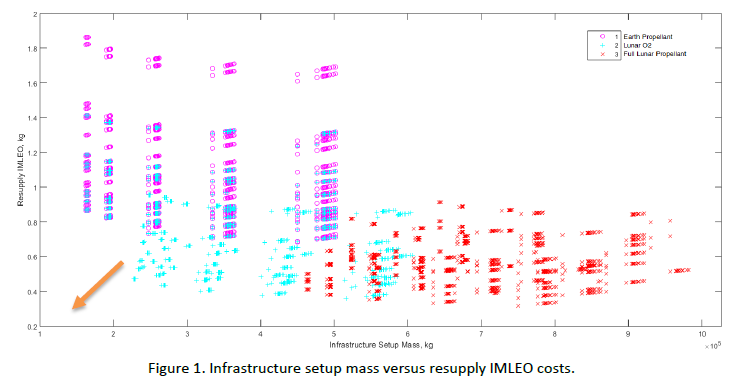
\includegraphics[width=0.7\textwidth]{InfraTrade}  %These are a bit too small to read
	\caption{Infrastructure Setup Mass Versus Resupply IMLEO Costs for Different ISRU Architecture Configurations.}
	\label{fig:infratrade}
\end{figure}

Figure \ref{fig:fulltrade} displays the design space for the science value of the missions versus the resupply IMLEO costs. The science value of the mission represents a research attempt to capture the utility of the mission, the third and final objective function. The Pareto frontier extends along the bottom and right sides of the design space indicating architectures that are efficient in terms of these two objective functions, being most efficient in the direction of the golden arrow.

\begin{figure}[h!]
	\centering
	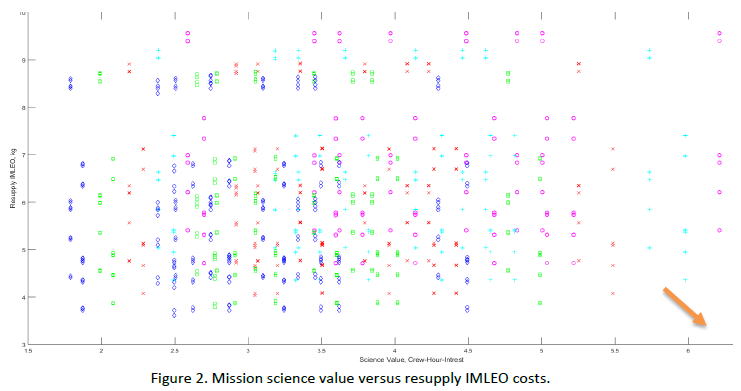
\includegraphics[width=0.7\textwidth]{fulltrade}
	\caption{Mission Science Value Versus Resupply IMLEO Costs.}
	\label{fig:fulltrade}
\end{figure}

Finally, three promising mission architectures from the Pareto frontier of Figure \ref{fig:fulltrade} were extracted and a sensitivity study was conducted regarding  the LH$_2$ Isp and NTR Isp factors. Figure \ref{fig:senstrade} displays the result of this study suggesting that the IMLEO resupply mass is highly sensitive to both improved  LH$_2$ Isp and NTR Isp, depending upon the level of Lunar ISRU in the mission architecture; this supports the further investigation of these factors through this research.

\begin{figure}[ht!]
	\centering
	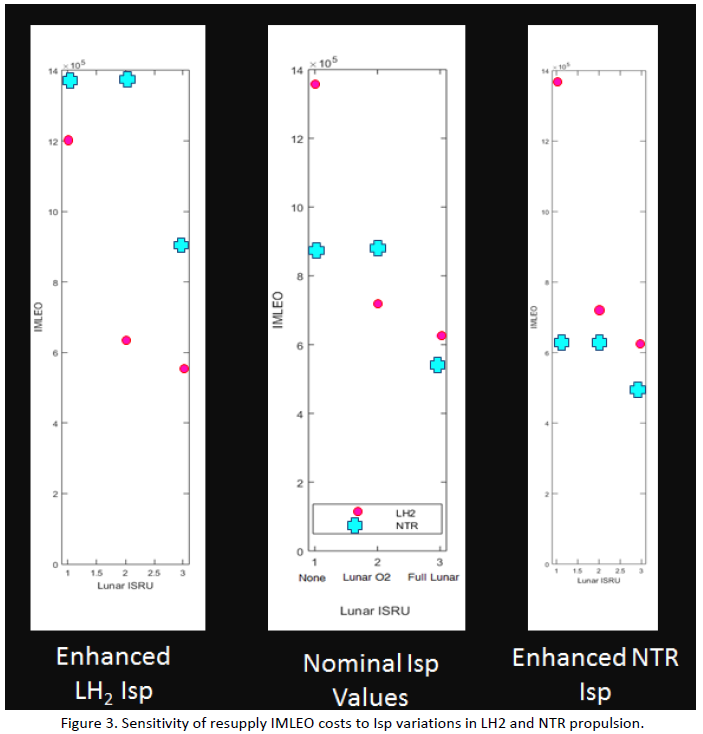
\includegraphics[width=0.5\textwidth]{improvetrade}
	\caption{Sensitivity of Resupply IMLEO Costs to Isp Variations in LH$_2$ and NTR Propulsion.}
	\label{fig:senstrade}
\end{figure}


\subsection{Initial Design}
Based on the DOE (section \ref{sec:single}.\ref{sec:DOE}) performed, an initial starting point for the optimizer may be determined by selecting a mission architecture that lies on or near the Pareto frontier “knee” point in Figures \ref{fig:infratrade} \& \ref{fig:fulltrade}. Reviewing the figures, architecture \#1400 was selected as the starting point for potential optimization algorithms. This design  consists of a promising architecture (low mass, high science value) and baseline technology parameters. Architecture 1400 has operating base location at Amazonis with photovoltaic power generation and 25\% of food grown in-situ. For the Isp efficiency factor it appears that enhanced Isp provides clear IMLEO benefits, but at potentially high developmental costs.

\begin{equation*}
\mathbf{x}=
\begin{bmatrix}
Isp_{LH_2}\\
Isp_{NTR}\\
\alpha\\
C_{surf}\\
C_{transit}\\
\end{bmatrix}
=
\begin{bmatrix}
\mbox{LH}_2\mbox{ Isp}\\
\mbox{Nuclear Thermal Rocket Isp}\\
\mbox{Architecture}\\
\mbox{Surface Crew Size}\\
\mbox{Transit Crew Size}\\
\end{bmatrix}
=
\begin{bmatrix}
465\\
950\\
1400\\
24\\
4\\
\end{bmatrix}
\end{equation*}

\subsection{Consolidated Objective}
In order to simplify the optimization to a single-objective problem, the scientific utility and cost were combined into a single objective, according to equation \ref{eqn:single}.
\begin{equation}
F = Utility/(Cost_{Development}+Cost_{Launch})
\label{eqn:single}
\end{equation}
This adds the cost of a single launch to the development cost, evenly weighting the two, and divides the scientific utility by this cost, reflecting the need to maximize the utility per million dollars.

\subsection{Coordinate Search}
\label{sec:coordinate}
From the results of the DOE, it was apparent that the full design space was highly non-linear, contained a variety of gaps and jumps due to the discrete nature of some design variables, and contained a variety of local maximum values. This suggested to the researchers that a gradient based optimization algorithm was not likely to successfully find the global maximum of the design space. As an alternative, a local coordinate search algorithm was developed by the researchers that conducted a steepest descent analysis and iterated to a local maximum point from some initial starting design. By using the results of the DOE to make educated guesses for the starting points, as well as running the coordinate search from multiple spatially distant starting points, the probability of finding the global minimum in the design space through relatively little computational effort could be made quite large. Furthermore, such a local coordinate search algorithm could be useful to refine results from the genetic algorithm presented in section \ref{sec:single}.\ref{sec:gasingle}. 

The pseudocode for the coordinate search algorithm is:
\begin{enumerate}
  \item Choose an initial design vector with guess values for all design variables
  \item For each design variable evaluate the objective at a forward and a backward design value (if a valid entry) while holding all other variables constant
  \item If a better objective results is found, move to the design vector corresponding to the best objective found and repeat from step 2
  \item If no better objective is found then terminate search and save final design vector and objective value
  \item Complete the coordinate search
\end{enumerate}

The algorithm works well the design problem on hand because it is able to efficiently search the space using knowledge of the ‘distance’ between each of the discrete alternatives while considering the bounds of the problem, a challenge for gradient based search approaches. The coordinate search will always converge on the same solution (in the same time) given the same initial starting point. Therefore, achieving sufficient coverage of the design space to ensure that the global maximum value is found requires controlling the number of initial guesses, the location of these initial guesses, and the structure of the design space. The following discussion will introduce how the coordinate search was tuned to the Mars 2040 design space to allow for rapid solution finding at low computational cost. 

Figure \ref{fig:heatmap} displays the full set of design variables and all levels of these variables. One primary way to increase the efficiency of the coordinate search, reduce the chance the algorithm will become stuck in a local maximum point, and reduce the number of initial guesses that must be attempted is to is to remove local maximums from the design space, or “smooth” the design space. This can effectively be completed for the coordinate search by ordering each of the design variables such that holding all other factors constant, the objective value will be monotonically increasing or decreasing with changes in the design variable being changed. While this approach does not capture the interaction affects between multiple design variables being changed simultaneously, it was found to be an effective first order approach to reducing the number of local maximums in the design space. The color coding in Figure \ref{fig:heatmap} represents a “heat map” of the results of this smoothing exercise where the darker green represents “better” solutions that maximize the objective of science value per dollar, while lighter areas and white areas represent “worse” solutions around some initial guess. It can be seen that the smoothing exercise roughly ordered each of the design variable entries.

\begin{figure}[ht!]
	\centering
	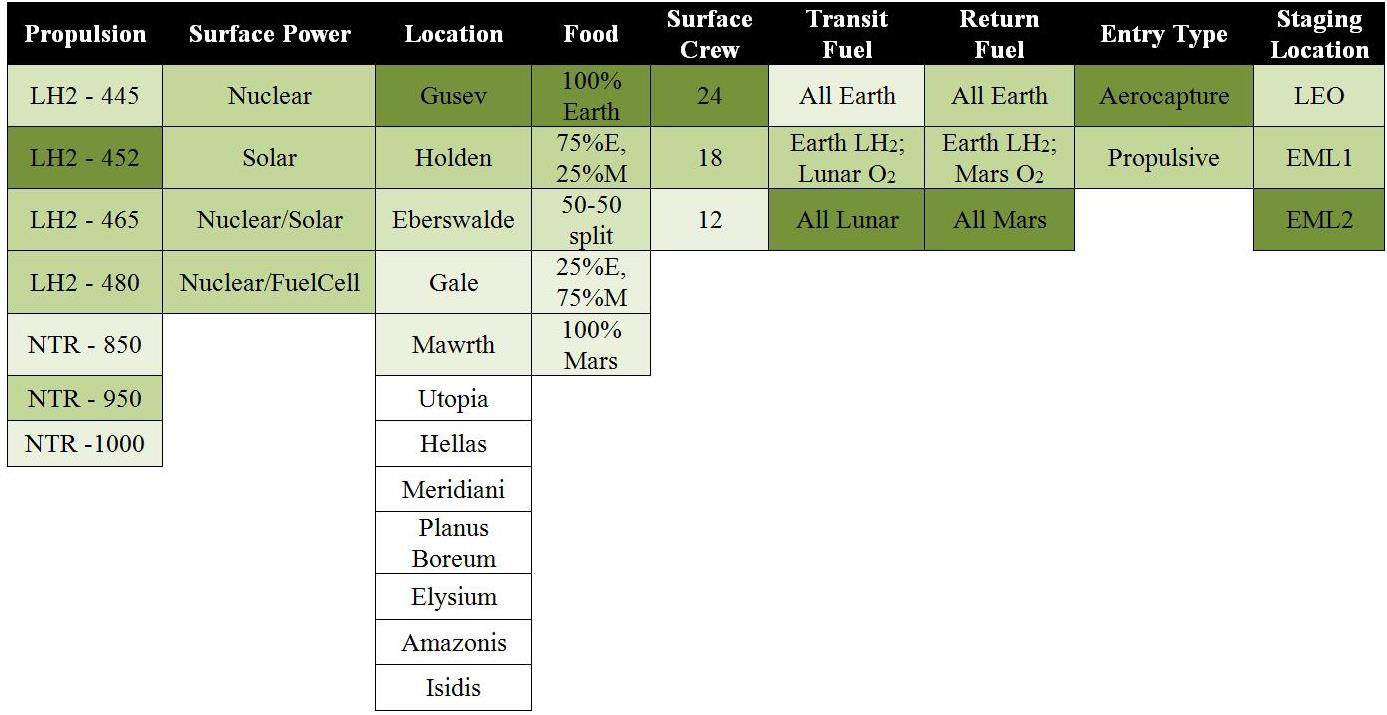
\includegraphics[width=1\textwidth]{DesignSpaceHeatMap}
	\caption{Full Mars 2040 Optimization Design Space with Heat Mapping to Display Smoothing Design Variables Around Local Point.}
	\label{fig:heatmap}
\end{figure}

Using the newly ordered design space, the coordinate search was executed from ten starting points (initial guesses) that covered the bounds of the design space as well as sampled the interior. As can be seen through the color coded optimal solution column in Figure \ref{fig:coordinateResults}, five different maximum values were found inside the design space. The four potential solutions indicated in orange were determined to be local maximums that had inferior ``value'' compared to the fifth maximum identified as the global maximum, indicated in green.

\begin{figure}[ht!]
	\centering
	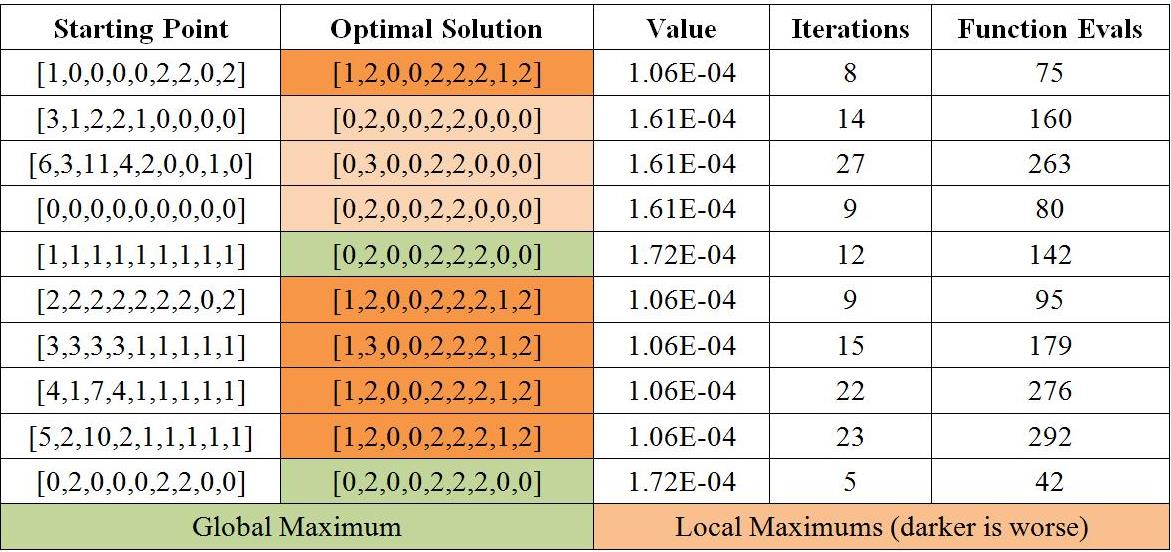
\includegraphics[width=.75\textwidth]{CoordinateSearchResults}
	\caption{Coordinate Search Results for Mars 2040 Design Space with Multiple Starting Point Guesses Revealing Local and Global Maximum Solutions.}
	\label{fig:coordinateResults}
\end{figure}

It should be noted that the design space contains a variety of local maximum values even after smoothing, but with the coordinate search started at multiple points around the design space it rather efficiently finds what appears to be the global maximum. The total computational requirements of the coordinate search with 10 initial starting points spread through the design space was 1604 function evaluations. The global maximum found corresponds to the following optimum architecture, X*, presented in Table \ref{tab:CoordResults}:

\begin{table}[t]
	\centering
	\caption{Results of Single-Objective Coordinate Search}
	\label{tab:CoordResults}
	\begin{tabular}{ll}
		\textbf{Design Variable} & \textbf{Optimization Result}\\ \hline
		Isp Improvement & 0.00 \\
		Food \% from Mars & 0.00 \\
		Propulsion Type & LH$_2$ \\
		Staging Location & LEO \\
		Transit Fuel Source & Lunar O$_2$, Lunar H$_2$ \\
		Return Fuel Source & Martian O$_2$, Martian H$_2$ \\
		Surface Crew Size & 12\\
		Entry Type & Aerocapture \\
		Site & Gusev Crater \\
		Surface Power Source & Nuclear/Solar\\
	\end{tabular}
\end{table}

%\clearpage
\subsection{Genetic Algorithm}
\label{sec:gasingle}

While the coordinate search function was able to determine the global maximum value in the search space with relatively few function calls required, the algorithm is not guaranteed to identify the global maximum and therefore may not be robust for use at other design points or for sensitivity studies. Furthermore, the coordinate search required pre-evaluation smoothing of the design space. In order to avoid the extra computational requirements of smoothing and numerous starting points, the single-objective problem was also run with a genetic algorithm optimization routine. The benefits of using a genetic algorithm include not requirement for design space smoothing, a much greater probability of converging on the global maximum in the presence of multiple local maximums, and a greater consideration of the entire design space during optimization.

Matlab's \mcode{ga} function was used to run this optimization, over the same design space as the coordinate search. After tuning the \mcode{ga} parameters to the problem at hand, the algorithm came to appreciably the same optimal solution, as shown in Table \ref{tab:GAsingle}. The final \mcode{ga} parameters are listed in Ttable \ref{tab:gasingleparams}, and the optimization algorithm converged in 53 generations. It was found that a population size of at least 40 individuals was necessary to consistently converge on the global maximum. With smaller population sizes, the algorithm frequently settled in a local minimum. As can be seen in Table \ref{tab:GAsingle}, while the coordinate search converged on the ``nuclear/solar' surface power source, the \mcode{ga} did no consistently settle between that option or the ``nuclear/fuel cell'' option. This difference indicates the strength of the coordinate search to find the absolute maximum, while the \mcode{ga} may find the region of the maximum but not necessarily the absolute architecture. Rescaling of the problem within the local region of the solution or adjusting the bounds of the \mcode{ga} dynamically could perhaps increase its accuracy in future work.


\begin{table}[h]
	\centering
	\caption{Single Objective Genetic Algorithm Parameters}
	\label{tab:gasingleparams}
	\begin{tabular}{lc}
		\textbf{Parameter} & \textbf{Setting} \\ \hline
		Population Size & 40\\
		Elite Count & 2\\
		Crossover Fraction & 0.85\\
		Tolerance & $1x10^{-6}$\\
	\end{tabular}
	\end{table}

\begin{table}[h!]
	\centering
	\caption{Results of Single-Objective Genetic Algorithm}
	\label{tab:GAsingle}
	\begin{tabular}{ll}
	\textbf{Design Variable} & \textbf{Optimization Result}\\ \hline
	Isp Improvement & 0.00 \\
	Food \% from Mars & 0.00 \\
	Propulsion Type & LH$_2$ \\
	Staging Location & LEO \\
	Transit Fuel Source & Lunar O$_2$, Lunar H$_2$ \\
	Return Fuel Source & Martian O$_2$, Martian H$_2$ \\
	Surface Crew Size & 12\\
	Entry Type & Aerocapture \\
	Site & Gusev Crater \\
	Surface Power Source & Nuclear/Solar \textit{or} Nuclear/Fuel Cell\\
	\end{tabular}
\end{table}

\subsection{Genetic Algorithm Verification}
The genetic algorithm parameters were tuned so as to produce consistent solutions in as few function calls as possible. To verify the solution of the GA was accurate, the solutions were compared to the findings of the coordinate search approach and found to be nearly identical, except for a differences in the surface power unit. The GA suggested a nuclear fuel cell power unit should be used while the coordinate search suggested a nuclear solar configuration. The influence of these two design variable options on the overall objective value was found to be nearly zero, and therefore the differences in the two were deemed acceptable. The GA is advantageous over the coordinate search as it does not require any previous knowledge of the design space (to conduct smoothing) and may be achieved with a single initial guess rather than requiring a diverse set of initial guesses by tried for convergence. These qualities make the GA idea for optimizing the Mars 2040 design space as if more design variables were added, the GA could effectively consider the non-linear interaction effects between variables and remove the need for local smoothing of the design space.

In future iterations of this work, the strongest optimization algorithm would be to use the GA for the initial, broad search of the entire design space. The coordinate search could then be executed using the solution from the GA as the initial guess in order to fine tune the solution and verify the solution was at the absolute maximum in the local area.

%\subsection{Comparison}

\section{Multi-Objective Optimization}
\label{sec:multi}
The Genetic Algorithm and Coordinate Search optimization techniques both converged on the same result, but these were run on a weighted sum combination of the two objectives. While this can give a good indication of the solution space, it cannot reveal differences in priorities, or allow the decision makers to make these trade off themselves, since there is only a single point of understanding.

As such, we switched to a multi-objective analysis in order to better understand the full solution space over which a decision maker would be interested in evaluating the trades.

\subsection{Multi-Objective Problem Space}
\label{sec:multiprob}
The objective was redefined from section \ref{sec:formulation}, to the following:

\begin{align*}
\label{eqn:mulitobj}
\mbox{max:}& &f_1(\boldsymbol{x})&=\bigg(2\bigg(\frac{2}{3}(EL)+\frac{1}{3}(PL)\bigg)+ (XG)\bigg(\frac{10}{15}\bigg)\bigg)*\text{CH}(\gamma)& \text{and}& \\
\mbox{min:}& &f_2(\boldsymbol{x})&=Cost_{Development}+Cost_{Launch} & &
\end{align*}

 with the following additional constraints:
 
\begin{align*}
\mbox{s.t.:}& & 25\%&\leq Food_{From Mars}\leq 75\% & &\\
& & 12 &\leq Crew_{Surface} \leq 30 & &\\
& & Crew_{Transit}&=ceil(Crew_{Surface}/3)& &\\
\end{align*}

The food constraint was added to force the solution to use a minimum amount of food grown on Mars, such that the technology to do so could be developed and tested. While Scientific Utility adequately captures much of the motivation to establish an outpost on Mars, it does not measure the desire to develop and improve the capability for off-earth exploration. Essentially, an additional constraint was added to achieve this ancillary objective of developing and utilizing a system to add farming to the space life support system.

The two crew size constraints are based on our reasonable expectation of development on the surface of Mars and operations of the settlement. The minimum population on the surface must be between 12 and 30; a range which captures an approximate minimum for a settlement and maximum possible population given resources needed to build up the settlement. We have also required that all crew members spend a maximum of three synodic periods on the surface before being replaced. With a crew replacement and resupply mission every synodic period, this is equivalent to having a transit crew equal to one third of the surface crew.

\subsection{Multi-Objective Algorithm}
Section \ref{sec:gasingle} showed that the genetic algorithm package in Matlab returned the same results as the custom coded coordinate search. Since this validated the effectiveness of the \mcode{ga} algorithm, we chose to continue to apply it as we transitioned to the multi-objective problem. Matlab's \mcode{gamultiobj} function uses the same optimization techniques, but allows for multi-objective solutions. It is also ready for parallelization, which provides a significant benefit to run-time, cutting it in half or more, depending on the machine. With a population size of 100, and almost 1000 generations, the final optimization run took 23.83 minutes on a dual-core machine, and would have reached close to an hour without parallelization.

\subsection{Pareto Frontier}
Figure \ref{fig:gamultipareto} shows the Pareto Frontier found with the \mcode{gamultiobj} algorithm. The orange diamond shows the utopia point, while the problem space on the pareto front is shown as magenta stars. A phenotypical distance function was applied, placing preference on design solutions that are well spaced in the objective space, rather than the design space.
\begin{figure}[h!]
	\centering
	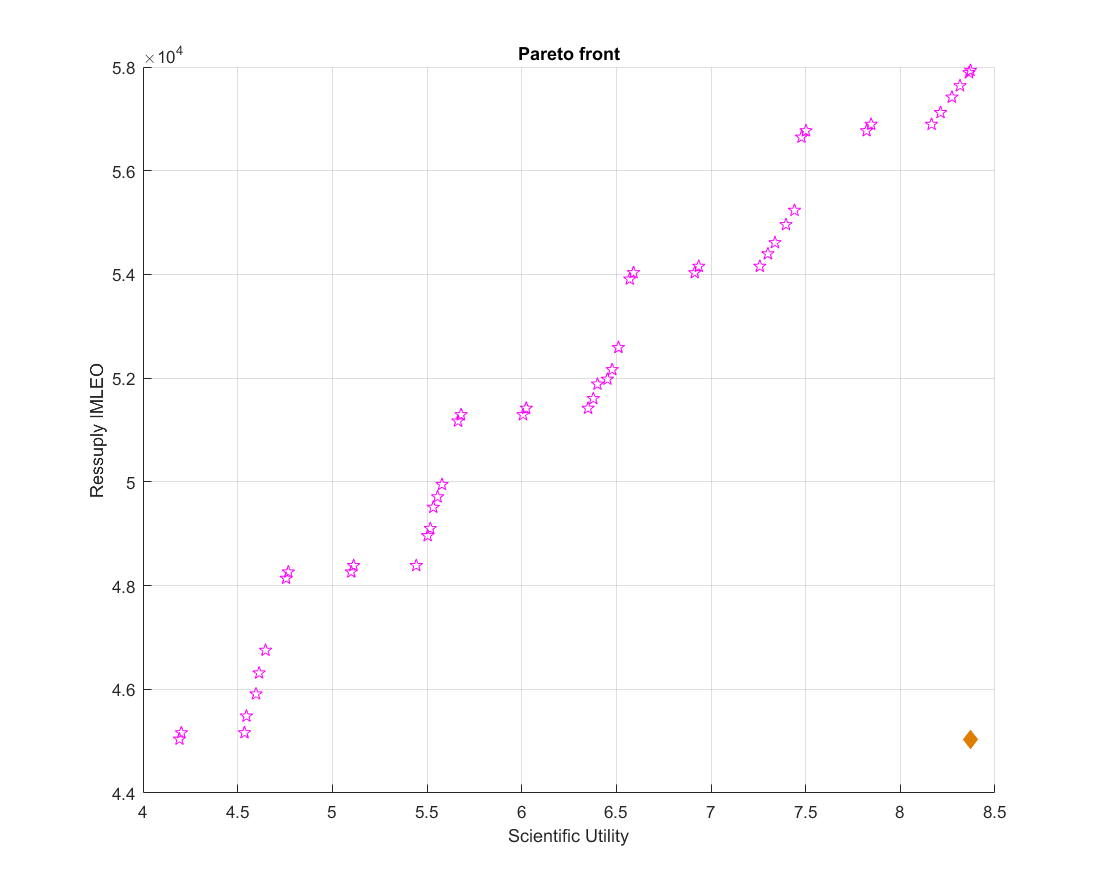
\includegraphics[width=0.5\textwidth]{ga-multi-pareto}
	\caption{Pareto Frontier from Multi-Objective Genetic Optimization}
	\label{fig:gamultipareto}
\end{figure}

This pareto frontier shows a clear pattern of steps, with curvature along each one.  The steps are created by the crew size variable. The transit crew is a large scaling factor on the transit spacecraft (and thus launch cost), and, as discussed in Section \ref{sec:multiprob}, the transit crew stays the same as the surface crew increases and approaches the ability for that transit crew size to rotate at least one third of the crew each launch.  As such, the cost jumps after that number is saturated (at a multiple of three), creating these dramatic steps in the pareto frontier.

\begin{figure}[htb!]
	\centering
	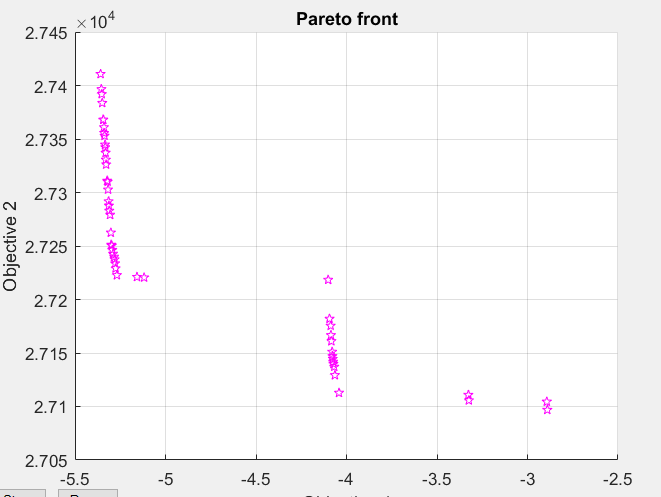
\includegraphics[width=0.5\textwidth]{pareto18}
	\caption{Pareto Frontier for a Fixed Surface Crew of 18}
	\label{fig:pareto18}
\end{figure}

Additionally, there is a slope to the lines connecting these stairs, and Figure \ref{fig:pareto18} shows that behavior more clearly by fixing the Surface Crew size to 18 members, and investigating that section in more detail.

\section{Final Recommendation}

Based on the findings of the multi-objective optimization, a design point was selected from the Pareto-dominant alternatives. The design vector is given in Table \ref{tab:GAmulti}. Due to the importance of crew number and synodic period, this design uses 18 surface crew to minimize the marginal cost of scientific return. The total cost, including launch and development of an advanced LH2 propulsion stage, is approximately \$48 billion dollars. With larger or small budget available, the crew could be scaled by multiples of three. The selected design also brings 65\% of food from Earth with the remaining 45\% grown on Mars. This serves to balance total launch cost and the science time available to the crew. Like the single-objective case, Gusev crater is chosen due to its high scientific interest factors and availability of resources for ISRU. 

\begin{table}[h!]
	\centering
	\caption{Results of Multi-Objective Genetic Algorithm}
	\label{tab:GAmulti}
	\begin{tabular}{ll}
	\textbf{Design Variable} & \textbf{Optimization Result}\\ \hline
	Isp Improvement & 0.12 \\
	Food \% from Mars & 0.45 \\
	Propulsion Type & LH$_2$ \\
	Staging Location & LEO \\
	Transit Fuel Source & Lunar O$_2$, Earth H$_2$ \\
	Return Fuel Source & Earth O$_2$, Earth H$_2$ \\
	Surface Crew Size & 18\\
	Entry Type & Aerocapture \\
	Site & Gusev Crater \\
	Surface Power Source & Nuclear\\
	\end{tabular}
\end{table}

Note that while this is our final recommendation, many designs along the pareto front would be very good choices as well. Clearly, a surface crew size that is a multiple of the stay duration, since that always provides a better utility for a marginally higher cost. Additionally, the weighting on the scientific utility calculation could have a significant impact on site selection and other architectural decisions.  While our assumptions resulted in this pareto optimal set, changes to the utility weightings could alter the optimal designs. However, the specific science priorities will be specific to the campaign planners, so these weightings are left to exploration, but this must be considered when selecting a final architecture.  

\section{Learnings and Future Work} 
The results show that the number of crew, the allocation of their time, and the relative costs of launch and technology development are important factors in designing a Martian surface outpost. 

Future work is planned to continue to investigate sensitivities to parameters which may be adjusted through additional development efforts. For example, the amount of time required to tend food crops drives the value of the mission. Augmenting the crew's ability with more automated crop tending systems could greatly increase the scientific value while maintaining launch costs at similar levels. Other follow-up analyses include investigated additional design variables such as ISRU efficiency, alternate locations, and surface stay time. Additional objectives to be investigated are initial emplacement costs, a more comprehensive set of development costs, and risk. Finally, the outpost architecture can also be evaluated in a more realistic context of a human exploration campaign by accounting for flexibility and commonality required over the next few decades.



\appendix
%\section{Master Table}
%\label{app:mastertab}


\section*{Acknowledgements}
The authors thank Dr. Olivier de Weck and the MIT 16.888 course staff including Drs. Ipek Basdogan, Caitlin Mueller, Sydney Do, and Darren Chang as well as the 2015 MIT \textit{Mars 2040} project team.

%% References
\bibliographystyle{aiaa}
\bibliography{./bib/aiaa}


\end{document}
